\documentclass{article}
\usepackage{amsmath}
\usepackage{graphicx}
\usepackage{color}
\usepackage{multicol}
\usepackage{float}

\begin{document}
\renewcommand\bibsection{\subsection{\refname}}
\title{\textbf{Creating two dimensional polymer configurations with the Rosenbluth algorithm}}
\author{Lennie de Roo and Selwyn Hanselman, \\
 \emph{Delft University of Technology}}
\date{\normalsize{April, 2015}}
\maketitle 
\noindent \hrulefill
\begin{abstract}
\nonindent In this project a simulation of polymer configurations was made. We used the pruned-enriched Rosenbluth method to grow a population of polymers by sequentially adding monomers. The interaction between monomers was modeled with the Lennard-Jones potential. The end-to-end distance of a polymer as a function of the number of monomers $N$ was found to scale with $N^{0.75}$.
\end{abstract}
\hrulefill
\begin{multicols}{2}
\subsection*{Introduction}
The behavior of polymers is a topic which is important in statistical mechanics \cite{Jos}\cite{Paper}.  For simulating the behavior it is desired to find the possible polymer configurations. An interesting quantity of polymers to look at is the end-to-end distance.
\subsection*{Simulation description}
For this simulation the polymers are modeled as existing of a chain of particles with a fixed distance between the particles (where the particles can be whole molecules). The model used assumes that the polymers are in a solution such that the polymers do not feel any interaction with other polymers. Furthermore the polymer segments are assumed to have a higher free energy when completely surrounded by solution instead of being close to another polymer segment. Now the only interaction a polymer has, is between its own segments and then only between the particles (the connection between the particles does not interact with anything). This interaction between two particles at a distance $r$ from each other, is in this simulation described by the Lennard-Jones potential:
\begin{equation}
 V_{LJ}=4\varepsilon\left[\left(\frac{\sigma}{r}\right)^{ 12}-\left(\frac{\sigma}{r}\right)^{6}\right]
 \label{eq:LennardJones}
 \end{equation}
Here $\varepsilon$ is the depth of the potential well (in this simulation set to $0.25$), and $\sigma$ is the distance at which the inter-particle potential is zero (in this simulation set to $0.8$). The distance between two subsequent particles is set to $1$. The different polymer configurations are found by growing the polymers particle by particle. To make sure that the configurations are not highly improbable, configurations with high energy are avoided. To do this  the \emph{Rosenbluth algorithm} can be used \cite{Jos}. 
\subsubsection*{Rosenbluth algorithm}
 \begin{figure*}[ht]
\centering
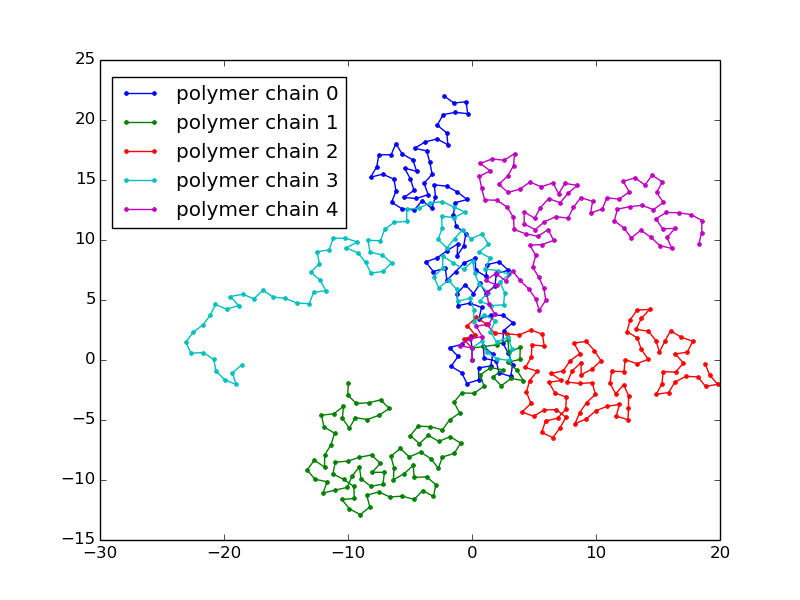
\includegraphics[width=10cm]{beterepolymerenplaatje.png}
\caption{The particle locations, and connections between the particles of 5 different polymers created with the Rosenbluth algorithm.}
 \label{fig:polymers}
\end{figure*} 
The Rosenbluth algorithm (in 2 dimensions) starts with a polymer consisting out of two particles, with the first particle on position (0,0), and the second one on position (1,0). The following particles are added one by one. In two dimensions the position of a new particle can be defined by the angle with the x-axis $\theta$, and the position of the previous particle (since the distance between the particles is fixed). Before a new particle is placed, a number (in this simulation 6) of optional places for this particle are investigated. These options are chosen by taking \emph{number of options} different angles, which have a random offset angle and are spaced by $\frac{2\pi}{\textrm{number of options}}$. Now one of these options $j$ is randomly chosen, where the options which add less interaction energy  $E(\theta_j)$ to the total configuration are more likely to be chosen: the probability for choosing angle $j$ for particle $l$ is  $\frac{w_{j}}{W}$ where $w_{j}=e^{\frac{-E(\theta_j)}{k_BT}}$ and $W=\sum_{j}e^{-\frac{E(\theta_j)}{k_BT}}$. The interaction energy $E(\theta_j)$ is found by calculating the Lennard-Jones potential (equation \ref{eq:LennardJones} between each previous particle with the new particle if it was set on position $j$ and summing these. This gives polymers which are very unlikely to cross themselves, and if one would plot a couple of these polymers this would result in an image like in figure \ref{fig:polymers}. However, the likely hood of most of the chains which are created this way is still very low. This is because in the population of created polymers, the chance that a certain configuration is created is not the same as its Boltzmann factor $Z=e^{\frac{E_{total}}{k_BT}}$ whereas it should. This happened due to the finite amount of investigated options for each added particle. Now it can be that polymers with a higher Boltzmann factor can have a lower probability to be present in the population than polymers with a lower Boltzmann factor. To make the probability of a polymer with a higher Boltzmann factor higher, the \emph{pruned-enriched Rosenbluth method (PERM)} can be used. 

\subsubsection*{PERM}
In the pruned-enriched Rosenbluth method, bad polymer configurations are removed from the population (pruning) and good configurations are copied (enriching). For knowing whether a configuration is a good or a bad one each one gets a weight factor. This weight factor of a configuration, is at the start of its growth defined as $1$. Then, by every addition it is multiplied by the factor $W=\sum_{j}w_j$. This is the factor the probability of a configuration was too low compared to the Boltzmann factor. When a configuration is removed or copied, its weight should not change. This can be achieved by when copying a certain configuration also halving the weight of both of the copies. When a configuration is deemed bad, it has a chance of a half to survive, and when it does its weight is multiplied by 2. This way the expectation value of the weight of this particular configuration stays the same. To keep a population that does not die out nor explodes with too many polymers, the pruning and enriching rate should be similar. Therefore the low limit under which the polymers have a chance to be removed and the up limit above which they are copied should be chosen carefully. It turns out that for the up limit $2.0*\frac{\textrm{Average weight}}{\textrm{weight at 3 particles}}$ is a good value, and for the low limit $1.2*\frac{\textrm{Average weight}}{\textrm{weight at 3 particles}}$\cite{Jos}. For the average weight only polymers with equal lengths should be compared. It turns out that it is more efficient to change limits at every step where a particle is added to the polymers in the population. However, it is easier to adjust the weights of the polymers instead. With some trial and error it was found that multiplying all the weights by a factor of $\frac{1}{0.55*\textrm{number of options}}$ gives a reasonable ratio for the pruning and enriching ratios. 

\subsubsection*{End-to-end distance}
The end-to-end distance of a polymer is the distance between the particles at the ends of the polymer chain. The average squared end-to-end distance of a polymer population of a single run is plotted against the number of particles in the polymer chains (figure \ref{fig:end2end}). In this figure also the amount of polymer chains is plotted. Also the theoretical scaling for the end-to-end distance against the number of particles from the literature $R^2=a(N-1)^{1.5}$ \cite{Jos}  is plotted, with $a$ chosen to fit the data. There is a good agreement between the theoretical fit and the calculated data from the simulation.
 \begin{figure*}[ht]
\centering
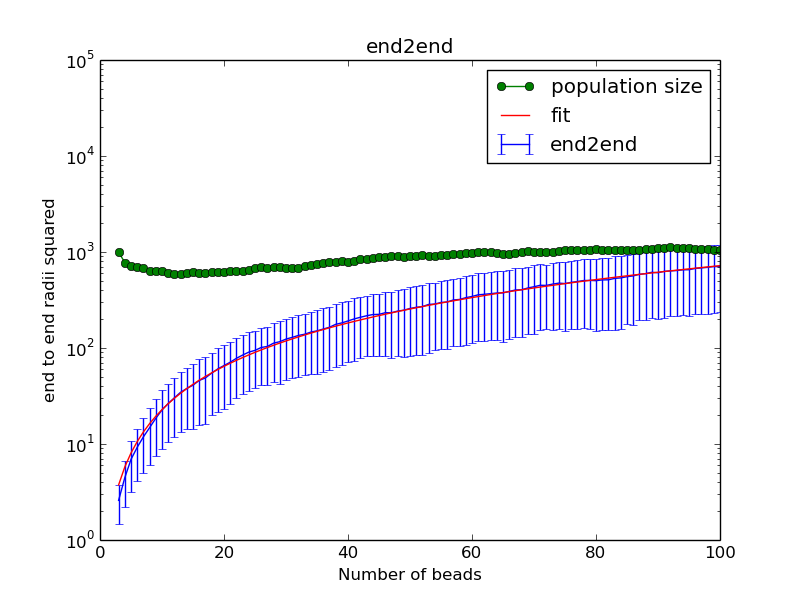
\includegraphics[width=\textwidth]{betereplot.png}
\caption{A plot of the average squared end-to-end distance of a polymer population starting with 1000 chains, plotted against the number of particles in a chain, which grows to 100 particles. At each addition step the population is pruned and enriched. Also the population size at each addition step is plotted, as well as the theoretical fit for the squared end-to-end distance against the number of particles in a polymer. }
 \label{fig:end2end}
\end{figure*} 
\subsection*{Conclusions}
The pruned-enriched Rosenbluth method  for finding the polymer configurations does find end-to-end data that corresponds well to the theoretical relation.
\begin{thebibliography}{9}
\bibitem{Jos} J.M. Thijssen,\emph{ Computational Physics}, Second edition, University Press, Cambridge, 2007
\bibitem{Paper} Nicolas Combe, Thijs J.H. Vlugt, Pieter Rein ten Wolde and Daan Frenkel, \emph{Dynamic pruned-enriched Rosenbluth method}, Molecular Physics, Vol. 101, No.11, 1675-1682, June 2003
\end{thebibliography}

\subsection*{Appendix}
The code for this simulation can be found at github.com/srhanselman/iccp-polymer, with the relevant files being:
\begin{itemize}
\item main2D.py
\item chain2D.py
\item listsofchains2D.py 
\item Potcalc2D.f90
\item plotter2D.py
\end{itemize}
\end{multicols}
\end{document}
